%%%%%%%%%%%%%%%%%%%%%%%%%%%%%%%%%%%%%%%%%%%%%%%%%%%%%%%%%%%%%%%%%%%%%%%%%%%%%%%%
\documentclass[presentation]{beamer} %\mode<presentation>{\usetheme{sapere}}
\usetheme{CambridgeUS}
\usecolortheme{orchid}

\definecolor{themeColor}{HTML}{295D98}

\setbeamercolor*{structure}{bg=black,fg=themeColor}

\setbeamercolor*{palette primary}{use=structure,fg=white,bg=structure.fg}
\setbeamercolor*{palette secondary}{use=structure,fg=white,bg=structure.fg!75}
\setbeamercolor*{palette tertiary}{use=structure,fg=white,bg=structure.fg!50!black}
\setbeamercolor*{palette quaternary}{fg=white,bg=black}

\setbeamercolor{section in toc}{fg=black,bg=white}
\setbeamercolor{alerted text}{use=structure,fg=structure.fg!50!black!80!black}

\setbeamercolor{titlelike}{parent=palette primary,fg=structure.fg!50!black}
\setbeamercolor{frametitle}{bg=structure.fg!10!white,fg=structure.fg!50!black!80!black}

\setbeamercolor*{titlelike}{parent=palette primary}


\usepackage[utf8]{inputenc}
\usepackage{amssymb}
\usepackage{graphicx}
\usepackage{subfigure}
\usepackage{multirow}
\usepackage{hhline}
\usepackage{amsfonts,amstext,amssymb,wasysym}
\usepackage{fancyvrb}
\usepackage{alltt}
\usepackage{textcomp}
\usepackage{url}
\usepackage{multimedia,pgf}
\usepackage{geometry}
\usepackage{listings}
\usepackage{framed}
\usepackage{cleveref}

\definecolor{Fuchsia}{HTML}{8C368C}
\definecolor{OliveGreen}{HTML}{3C8031}

% Code highlighting
\newcommand{\il}[1]{{\it \textcolor{gray}{// #1}}} % inline comment
\newcommand{\km}[1]{\textcolor{purple}{#1}} % key mechanism primitives
\newcommand{\ex}[1]{\textcolor{blue}{#1}} % external imported Java values
\newcommand{\fc}[1]{\textcolor{Fuchsia}{#1}} % field calculus calls
\newcommand{\fn}[1]{\textcolor{blue}{#1}} % building block / function calls
\newcommand{\vb}[1]{\textcolor{OliveGreen}{#1}} % variables
\newcommand{\str}[1]{\textcolor{darkgray}{#1}} % strings

\newcommand{\bral}{\textrm{{\tt {\char '173}}}\,}
\newcommand{\brar}{\textrm{{\tt {\char '175}}}}
\newcommand{\var}{\texttt{x}}
\newcommand{\asgK}{~\texttt{=}~}
\newcommand{\letK}{\texttt{let}~}
\newcommand{\tupK}[1]{\texttt{[}#1\texttt{]}}
\newcommand{\lambdaK}[2]{\texttt{(}#1\texttt{)->}#2}
\newcommand{\bodyK}[1]{\bral\! #1\!\brar}
\newcommand{\dotK}{\texttt{.}}
\newcommand{\applyK}{\texttt{apply}}
\newcommand{\mname}{\ex{\texttt{m}}}
\newcommand{\aname}{\ex{\texttt{\#a}}}
\newcommand{\repK}[3]{\texttt{\fc{rep}(#1<-#2)}#3}
\newcommand{\ifK}[3]{\texttt{\fc{if}}(#1)#2\,\texttt{\fc{else}}\,#3}
\newcommand{\muxK}[3]{\texttt{\fc{mux}}(#1)#2\,\texttt{\fc{else}}\,#3}
\newcommand{\nbrK}[1]{\texttt{\fc{nbr}}#1}

\title[Gillespie's SSA to Integrate DES and MABS]{Extending the Gillespie's Stochastic Simulation Algorithm for Integrating Discrete-Event and Multi-Agent Based Simulation}

\author[Montagna, Omicini, Pianini]{
Sara Montagna, Andrea Omicini, \textbf{Danilo Pianini}\\
\texttt{{\footnotesize \{sara.montagna, andrea.omicini, danilo.pianini\}@unibo.it}}}


\institute[UNIBO]
{\textsc{Alma Mater Studiorum}---Universit\`a di Bologna a Cesena}

\date[2015-05-15 MABS]{The XVI International Workshop on Multi-Agent Based Simulation\\
\scriptsize May 5, 2015 - Istanbul, Turkey
}

\pgfdeclareimage[height=0.625cm]{university-logo}{imgs/logo}
\logo{\pgfuseimage{university-logo}}


\begin{document}


%===============================================================================
\frame[label=coverpage]{\titlepage}
%===============================================================================

\section*{Outline}
%===============================================================================
\frame{\tableofcontents}



%===============================================================================
\section{Background}
%===============================================================================

%-------------------------------------------------------------------------------
\subsection{Discrete Event Simulation (DES)}
%-------------------------------------------------------------------------------


\begin{frame}{DES}

\ldots The most used approach in the simulation mainstream
\begin{block}{}
	\begin{itemize}
    		\item Instantaneous events responsible for the changes in the system state
    		\item In between events, no change to the system is assumed to occur
    		\item Different events cannot be simultaneous
		\item It is normally very efficient since it allows to jump in time from one relevant event
	\end{itemize}
\end{block}

		
\emph{Defining a DES means to model the behaviour of a system as an ordered sequence of non-continuous events, by specifying for each of them the \emph{perturbations} in the system state it provokes, and the exact point in time when it has to be triggered. }

\end{frame}


%-------------------------------------------------------------------------------
\subsection{Agent Based Modelling (ABM) and Simulation (MABS)}
%-------------------------------------------------------------------------------

\begin{frame}{MABS}

\ldots Introduced as a novel and alternative approach to Discrete Event Simulation (DES) and to Systems Dynamic (SD)

\begin{block}{}
	\begin{itemize}
		\item More than a simulation method...it is a \textbf{philosophy}...    
    		\item ABM models the system at the \emph{micro-level}
		\begin{itemize}
			\item active entity are autonomous and interacting agent, 
			\item dynamic environment
			\item global system-level behaviour as a result of the agent-to-agent interactions
		\end{itemize}
	\end{itemize}
\end{block}

\begin{block}{The simulation platform}
	\begin{itemize}
		\item Various platforms were developed for the purpose \cite{simulationtoolkits-survey}, 
		\begin{itemize}
			\item  tools for developing, editing, and executing ABM, as well as for visualising the simulation dynamic. 
		\end{itemize}
		\item How do they operate over a timeline?
		\item How are agents and environment behaviours coupled and scheduled?
	\end{itemize}
\end{block}


\end{frame}


\begin{frame}{Crucial Issue: Time}
\textbf{How to deal with the evolution of time?}

\begin{block}{Continuous approaches}
	\begin{itemize}
		\item Rare
		\item Specifically used for modelling the endogenous dynamic of the environment coupled with discrete agent internal processes. 
	\end{itemize}
\end{block}

\begin{block}{Discrete approaches}
	\begin{itemize}
		\item Time-driven	
		\begin{itemize}
			\item most widely used
			\item fixed time steps
		\end{itemize}
		\item Event-driven
	\end{itemize}
\end{block}

\end{frame}



%===============================================================================
\section{Motivation}
%===============================================================================

\begin{frame}{Two intuitions}
  \begin{block}{Unique conceptual framework}
    Event-driven systems and multi-agent systems are amenable of a coherent interpretation within a unique conceptual framework
  \end{block}
  \begin{block}{Powerful simulation framework}
    From the integration of Discrete Event Simulation (DES) and Multi-Agent Based Simulation (MABS) \cite{meyer-mabs2014}
  \end{block}
\end{frame}

\begin{frame}{Motivation: why not  time-driven?}

  \begin{block}{Efficiency}
    \begin{itemize}
      	\item Time passes fixed time steps
        \begin{itemize}
          	\item even if no action changes the state happen in between
	\end{itemize}
      	\item Carefully choice of temporal granularity
      	\begin{itemize}
      		\item low granularity may ruin results
		\item high granularity may lead to a waste of computational resources
	\end{itemize}
    \end{itemize}
 \end{block}
  
  \begin{block}{Accuracy, validity, coherency}
    \begin{itemize}
      \item All the events happening in the same $\Delta{}t$ are executed together
        \begin{itemize}
      		\item possible loss of order and changes on the system outcome
		\item to be as close as possible to the MAS paradigm, actions and interactions should be conducted concurrently
	 \end{itemize}
    \end{itemize}
  \end{block}
  
  \begin{block}{Congruence}
    \begin{itemize}
      \item  Simultaneous updates of system entities is far from reality
    \end{itemize}
  \end{block}

\end{frame}

%===============================================================================
\section{A Unified Stochastic Computational Model}
%===============================================================================

\begin{frame}{Gillespie's SSA as an event-driven algorithm}
  \begin{block}{Gillespie's algorith}
    \begin{itemize}
      \item Gillespie \cite{gillespie1977} first proposed an event driven stochastic simulation algorithm (SSA) for the exact stochastic simulation of chemical systems
      \item Gibson and Bruck \cite{gibson2000} improved its performance
      \begin{itemize}
	\item Next reaction selection not by propensity (function of concentration of reagents and a markovian rate) but by generated putative times
	\item Dependency graph meant to update only the events whose scheduling time might have changed because of other events
      \end{itemize}
      \item Building on their work, we extended the algorithm in order to be able to shift from the world of chemistry to the richer MABS world
    \end{itemize}
  \end{block}
\end{frame}

\subsection{Model}
\begin{frame}{Generalised chemistry}
\begin{block}{Pure chemistry vs. agent-based systems}
\begin{itemize}
 \item Single, static compartment versus multiple, possibly mobile, and interconnected agents whose ability to communicate may depend on environmental and technological factors
 \item Molecules are described by concentrations (an integer), agents may carry and process any kind of data
 \item Reactions ``scheduling'' in nature follows a Poisson distribution whose rate equation depends on reagents' concentration \cite{gillespie1977}. Events in an agent-based simulation may be influenced by any of the environment components and follow any probability distribution (triggers, timers, events with memory)
 \item Agents live in an environment, such abstraction is absent in chemistry
\end{itemize}
\end{block}
Yes, it is a nicely big leap
\end{frame}

\begin{frame}{Close the gap: environment}
  \begin{figure}
    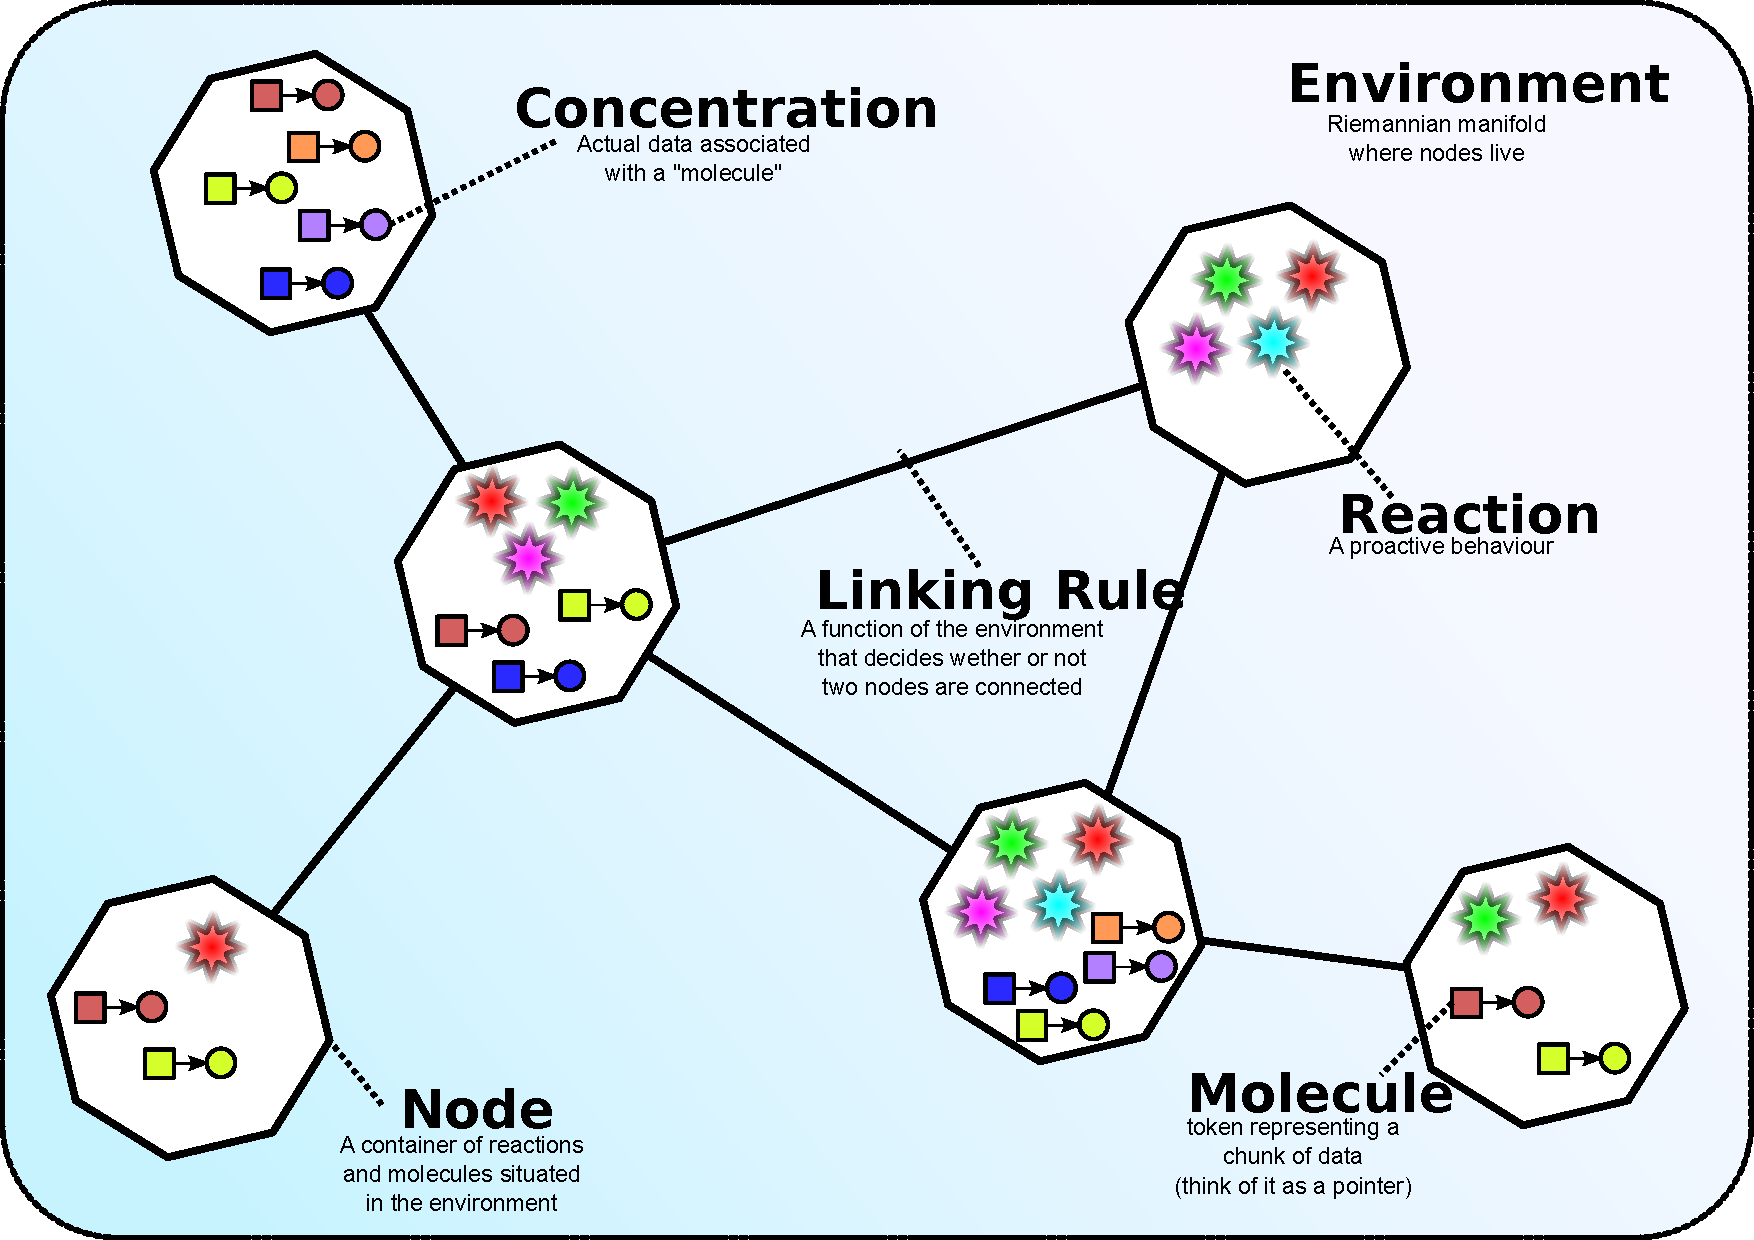
\includegraphics[
%       width=\textwidth,
      height=0.8\textheight
      ]{imgs/model} 
  \end{figure}
\end{frame}

\begin{frame}{Close the gap: reactions}
  \begin{figure}
    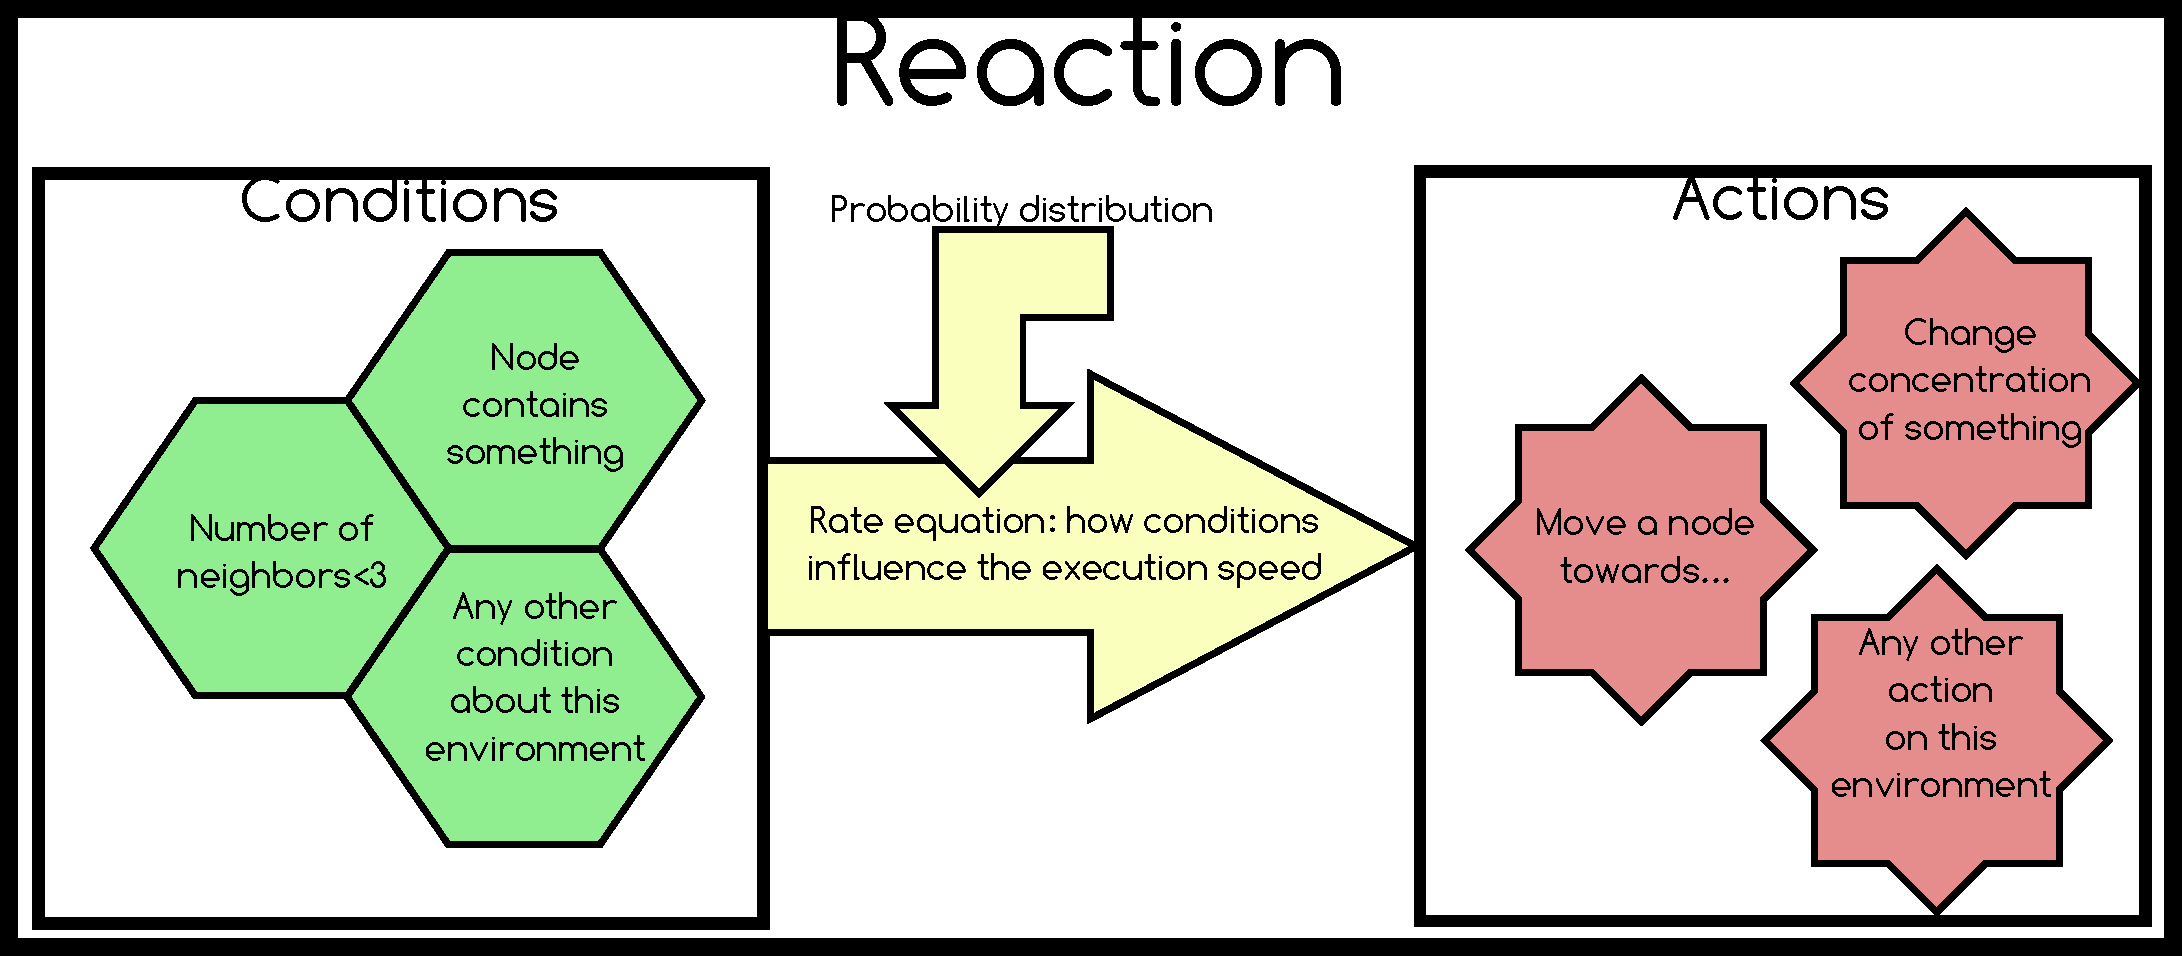
\includegraphics[
      width=\textwidth,
%      height=0.8\textheight
      ]{imgs/reaction} 
  \end{figure}
\end{frame}

\begin{frame}{Flexibility and data types}
  \begin{block}{Abstract Concentration}
    \begin{itemize}
    \item Concentration can be any data type
      \begin{itemize}
        \item Pick integers, the result is a simulator for (bio)chemistry, with multiple intercommunicating compartments situated in an environment \cite{drosophila}
        \item Pick ``set of tuples matching a tuple template'', the result is a simulator of network of programmable tuple spaces
        \item Pick ``any object'', the result is flexibile enough to simulate a network of devices running their own program \cite{protelis}
      \end{itemize}
    \item For each type of concentration, a specific set of legal conditions and actions can (must) be defined
    \item All the other entities can be defined in a generic fashion, and reused 
    \end{itemize}
  \end{block}
\end{frame}

\subsection{Engine}

\begin{frame}{Extended SSA phase 1: pick the next event}
  \begin{block}{How to select the next event?}
    \begin{itemize}
      \item Most high-performance SSAs presume an underlying model that only includes memoryless events \cite{slepoy2008}
      \item Gibson/Bruck's ``next reaction'' uses putative times instead
      \item We extended it adding support for addition and removal of events at runtime
      \begin{itemize}
        \item Agents may join and leave the system at runtime, new agents may be equipped with novel behaviours
      \end{itemize}
    \end{itemize}
  \end{block}
\end{frame}

\begin{frame}{Extended SSA phase 2: dependency management}
  \begin{block}{How to select the next event?}
    \begin{itemize}
      \item The dependency graph is key for the high performance of SSAs \cite{slepoy2008}
      \item In general, it is very hard to build a dependency graph in an open environment composed of multiple entities
      \item We extended the original concept of (static) dependency graph with:
      \begin{itemize}
        \item Events can be added and removed at runtime, the graph is dynamically updated
        \item Execution contexts: \texttt{local}, \texttt{neighborhood}, \texttt{global}
        \item Separation of influencing context and context of influence (input and output)
        \item Overall, the dependency graph is greatly pruned, with positive impact on performance
      \end{itemize}
    \end{itemize}
  \end{block}
\end{frame}


%===============================================================================
\section{Case study}
%===============================================================================



%-------------------------------------------------------------------------------
\subsection{A possible implementation: Alchemist platform}
%-------------------------------------------------------------------------------

\begin{frame}{Alchemist}
  \begin{block}{Chemical-inspired meta simulator}
    \begin{itemize}
      \item Based on the machinery already described
      \item Java written
      \item Provides out of the box support for simulating distributed programmable tuple spaces and Protelis \cite{protelis} devices
      \item Supports mobility and complex environments, both indoor and outdoor (with data from OpenStreetMap)
      \item Available as Maven artifact (\texttt{it.unibo.alchemist:alchemist})
    \end{itemize}
  \end{block}
\end{frame}

\begin{frame}{Architecture}
  \begin{figure}
    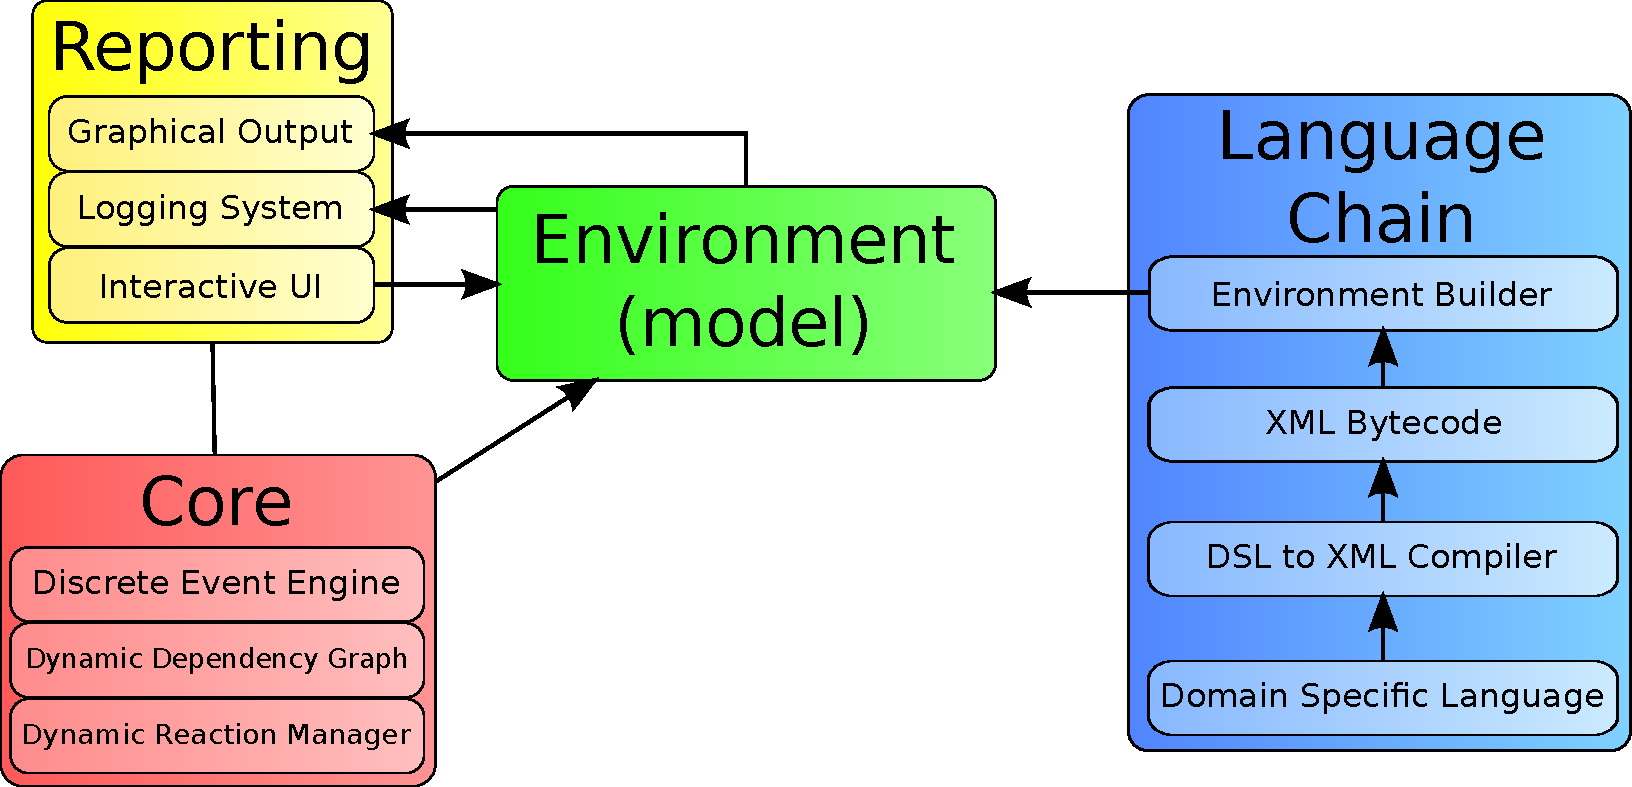
\includegraphics[width=\textwidth]{imgs/architecture} 
  \end{figure}
\end{frame}


%-------------------------------------------------------------------------------
\subsection{Example scenario: context sensitive crowd steering in a urban environment}
%-------------------------------------------------------------------------------

\begin{frame}{Crowd-sensitive user steering in London}

\begin{figure}[bt]\centering
  \subfigure[Initial]{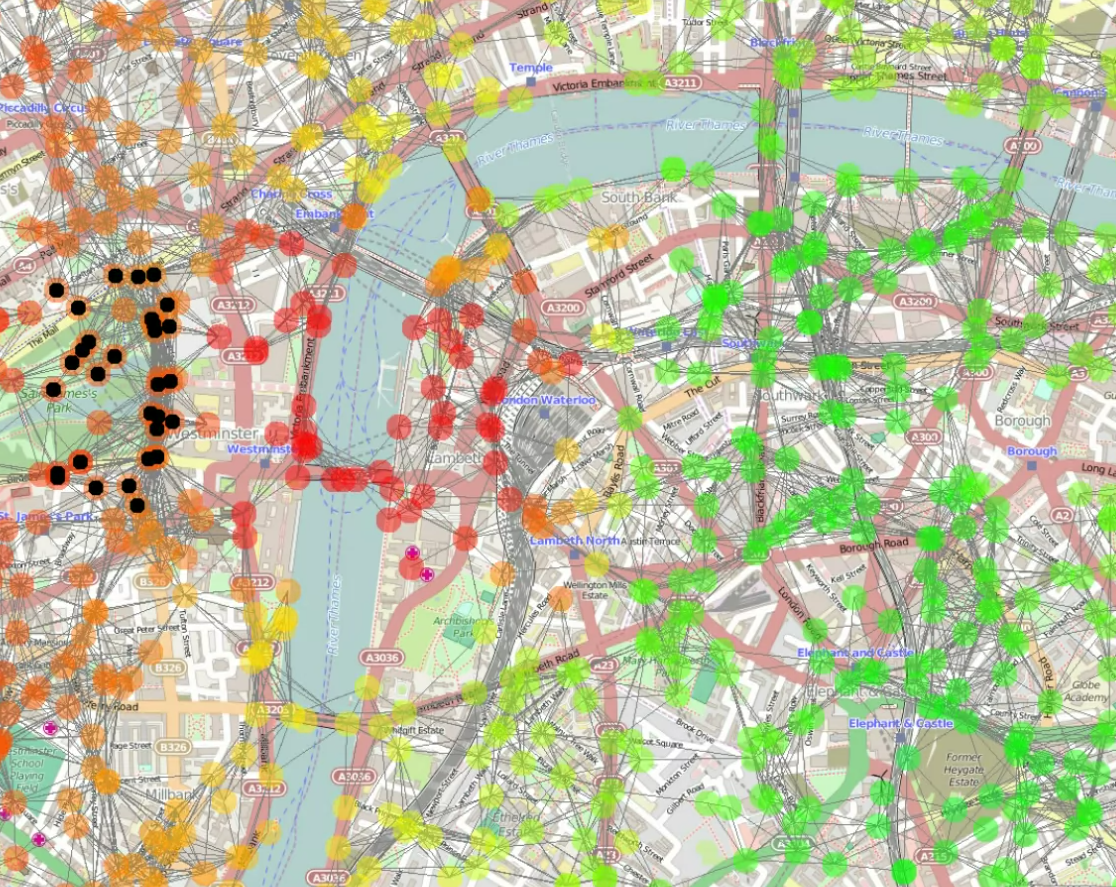
\includegraphics[width=0.32\textwidth]{imgs/london0}}
  \subfigure[Ongoing]{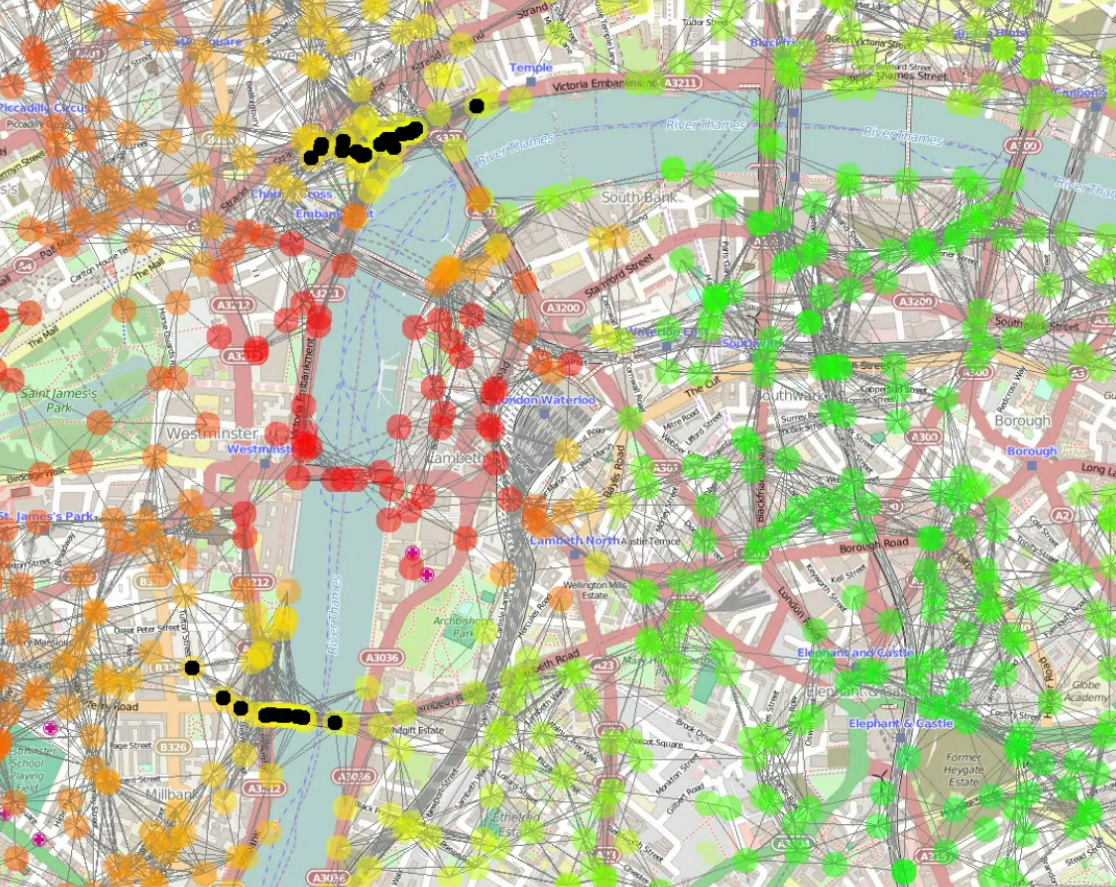
\includegraphics[width=0.32\textwidth]{imgs/london1}}
  \subfigure[Near-end]{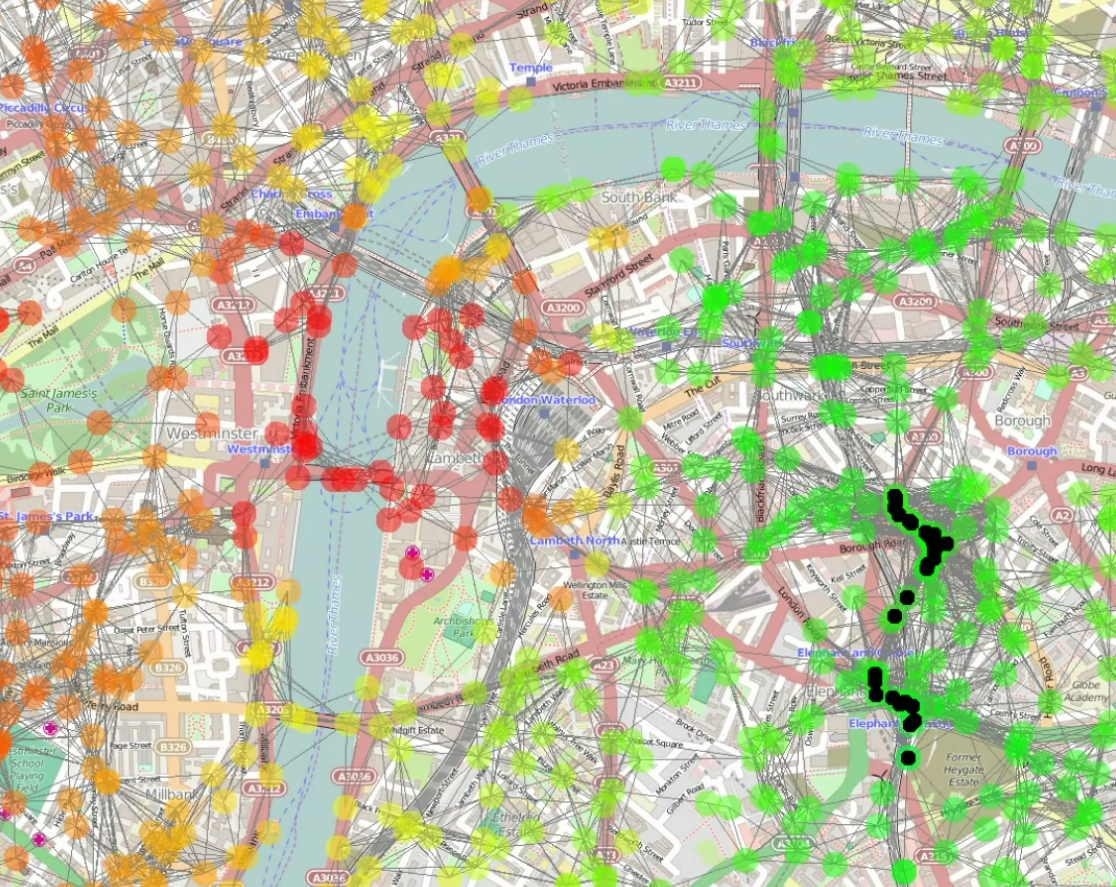
\includegraphics[width=0.32\textwidth]{imgs/london2}}
  \caption{Three snapshots of the simulation. Our altered distance metric (the gradient) goes from green (most favourable and close to destination) to red (unpleasant or far from destination). Agents (in black) climb this structure towards greener values.}
\end{figure}

\end{frame}



\section{Conclusion}
\begin{frame}{Conclusion}
  \begin{block}{Integration of DES and MABS}
    \begin{itemize}
      \item We adopted an extension of Gillespie's SSA as stochastic event-driven algorithm
      \item We extended it to support the inherent complexity of multiagent systems, still retaining the performance optimisations
      \item We extended the chemical model towards higher flexibility, introducing the enviromemnt, generalising the concept of reaction and allowing arbitrary data to be a ``concentration''
      \item We implemented those concepts inside the Alchemist framework
      \item A non-trivial example was provided: crowd steering in London
    \end{itemize}
  \end{block}
\end{frame}



\section*{\refname}
%===============================================================================
\begin{frame}[allowframebreaks]
%\begin{frame}[t,allowframebreaks]
  \frametitle{\refname}
  \scriptsize
  \bibliographystyle{alpha}
  \bibliography{bibliography}
\end{frame}
\section*{\refname}




\end{document}